
%\subsection{Extending the Tor protocol}
%
%We extend the Tor routing protocol described in Tor's
%specifications~\cite{dingledine2018tor} and exploit Tor's leaky-pipe circuit
%topology\footnote{``Leaky pipe'' refers to the ability of the user to direct
%  traffic that ends at an intermediate hop along the circuit} to exchange
%payment information with each hop of the circuit. We introduce two new control
%cell types: one link-level cell and one relay-level cell. The link-level cell is
%used to exchange information related to the payment protocol between the Tor
%client and its guard relay while the relay-level cell is used for the middle
%relay and the exit relay. This subtype of relay cell is comprised of a payment
%header denoting the type of payment cell, followed by a payload of payment
%data. To an outside observer, payment cells are indistinguishable to normal
%relay cells. Figure~\ref{fig:relay_command_mt_structure} shows the internal structure of the cell.
%\begin{figure}[h]
%    \centering
%    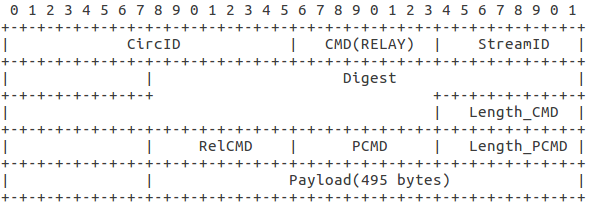
\includegraphics[scale=0.38]{images/payment_cell_header.png}
%    \caption{Relay Payment Cell --- Cell definition specifying the structure of
%      a moneTor payment cell. Note: a block that appears blank and empty is in fact the continuity of the previous row}
%\label{fig:relay_command_mt_structure}
%\end{figure}
%
%All the bytes starting from StreamID (included) are onion encrypted. RelCMD is
%set to RELAY\_COMMAND\_MT, PCMD is the payment command which is different for
%each step of the payment protocol. If some message overflows the payload
%available length (495 bytes), we queue multiple cells of the same PCMD and
%buffer them on the receiver side to unpack the whole message.

\subsection{Pre-built Channels}
By default, Tor attempts to pre-build circuits in order to reduce latency once a
user wishes to create a data stream. Much like circuits, moneTor payment
channels are high in initial latency because of the many in-out messages in the
protocol. We therefore exploit the same strategy currently used in circuit
establishment by allowing payment channels to be preemptively set up and
established on clean pre-built circuits. This dramatically reduces the effective
time to first payment. Unfortunately, excessive establishment of preemptive
channels will eventually afflict the network with unused overhead. Our
implementation features a rudimentary prediction strategy that attempts to
balance this trade-off by anticipating the number of needed channels using
historical usage information in a similar way Tor anticipates the need for a
fresh circuit. The effectivness of preemptively established channels is analyzed
in Section~\ref{sec:experimentations}, and is expected to make the payment
confirmation time matching the round-trip-time of the client-relay connection.

%However, our approach may not be sufficiently optimized and further
%work on this front is warranted.
%
%\subsection{Network Scalability}
%\label{subsub:scalability}
%%\td{TODO: describe scalability of intermediary system and any networking
%%  bottlenecks that might arise such as port limits, etc.}
%
%In our design, we are concerned with memory consumption, kernel socket
%consumption and CPU consumption. Our choice for a tripartite protocol
%effectively shifts the memory consumption of opened and idle micro
%channels to the intermediary nodes of the network.
% 
%% A more basic setup
%%whereby each Tor client maintains a micropayment channel with each
%%relay would incur an $O(n*m)$ cost with
%%respect to channel management complexity, with $n$ the number of Tor clients and $m$ the number of relays. By engineering an additional
%%intermediary layer, the complexity of moneTor channel connections is
%%reduced to $O(n+m)$. In our implementation, intermediary relays do not
%%participate in routing user streams and are tasked only with providing
%%payment channel services. Intermediaries devote the full extent of
%%their computational resources toward this task, allowing only a few
%%strong nodes to handle all of channel management needs of the network.
%
%Interactions between parties are realized within Tor circuits to allow
%multiplexing of circuits over the same TCP connection. This also protects the
%identity of the client and its chosen circuit against identification by the
%ledger or the intermediary.
%%\footnote{We assumed no side-channel exploitation in
%%  this work but do discuss timing attacks in
%%  Section~\ref{sec:limitations_futurework}.}. 
% As a result, the intermediary and
%the ledger must have a number of available sockets higher than the number of
%relays in the network in the worst case. Since this limit is in line with Tor's
%current assumption (i.e., any relay has available sockets to connect to every other relay), our design inherits the same socket consumption scalability
%of the greater Tor network.

\subsection{Prioritized Traffic}
\label{subsub:prioritized}

%The final component of our network-oriented design addresses the need to deliver
%prioritized bandwidth given an explicit signalling of premium or nonpremium
%traffic. Our objective is to provide a tunable range of prioritization while
%incurring as little cost as possible to average global performance. In our
%design, the chosen value is enforced network-wide by the directory authorities
%in order to avoid partitioning of the anonymity set. 
Traffic scheduling is perhaps the most intuitive mechanism with which to
implement prioritization. However, we found that local scheduling decisions on
each relay for priority do not work well with the current state of the Tor
network, which precludes out-of-the-box scheduling approaches based on
DiffServ~\cite{dovrolis1999case} and EWMA~\cite{tang2010improved}. Intuitively,
this is a direct result of the evolution of the Tor network capacity over recent
years. Due to the growth in bandwidth across guard and middle relays, the
network now sees the most congestion between the exit relay and final
destination. In our analysis of scheduling under a simulated modern Tor
topology, we found that relays were able to instantaneously flush their queues
at each write event, rendering any attempt at local scheduling to be
ineffective. We believe that these results, detailed in
Appendix~\ref{sec:scheduling}, may suggest a need for a separate comprehensive
study of network prioritization mechanisms.

Consequently, we turn the alternative strategy of prioritizing traffic through
Tor's internal control-flow window sizes, which conversely tends to be more
accurate with lower internal congestion~\cite{archive-2009-mail,
  kiraly2008solving}. Indeed, since local decisions inside the scheduler at a
particular relay may fail to achieve priority, designing priority as a global
function of the circuit may help. Recall that edge nodes regulate the traffic
flux in either direction using a set of flow control windows. Roughly speaking,
these windows determine space allotted to each circuit on a relay's scheduling
queue, which in turn is positively correlated with effective bandwidth. We
implement our prioritization scheme by statically readjusting the window maximum
sizes once according to the following formula (both Circ window and Stream
window).
\begin{equation}
  window' = window(1+ \alpha(premium / pr\% - 1))
  \label{eq:flow}
\end{equation}
Here, a circuit is marked as prioritized by the bit $premium \in \{0, 1\}$. The
tunable priority benefit $\alpha \in [0, 1]$ defines the proportion of the
non-premium capacity that we wish to transfer to premium clients. By accounting
for $pr\% \in [0,1]$, the fraction of premium to nonpremium clients, we can keep
the total flow capacity constant. This design decision means that the memory
consumption at relays induced by processing cells should stay constant as well.

Even if most relays are able to flush all queues at each write event, some
relays may still be congested within the Tor network. In this case, modifying
Tor's overlay flow control would not achieve priority since the cells are stuck
within the congested relay's queues. To overcome this issue, we modify EWMA with
a simpler linear scaling factor that favors paid circuits.

\begin{equation}
  A_{t + \Delta t} = A_t \times 0.5^{\Delta t/H}
\end{equation}
\begin{equation}
  A'_{t + \Delta t} = A_{t + \Delta t} / \beta + C_{t, t + \Delta t}
\end{equation}

Defined in Tang and Goldeberg's original paper~\cite{tang2010improved}, $A$ is a
variable score used to sort circuits such that the circuit with the lowest $A$
is always next on the scheduling queue. $C$ is the number of cells relayed
within $\Delta t$, the time since the previous observation, and $H$ is a global
representing the half-life decay interval in the score. Our added term, $\beta
\in [1, \inf)$, is a tunable parameter such that $Bandwidth_{premium} =
  Bandwidth_{nonpremium} \times \beta$ for any given circuit under ideal
  conditions.

%Our policy may be implemented in one of two ways. First, each node could track
%the $premium\%$ locally and dynamically adjust their own windows. This
%introduces a considerable amount of added complexity with unclear consequences
%on network performance. A more sound approach calls for the Tor authorities to
%track the global value for $premium\%$ and periodically broadcast static flow
%control windows to be used by the entire network. We adopt the latter approach
%in this iteration of moneTor.

\paragraph*{Interlude.} This concludes the design of the moneTor framework. In
the proceeding sections, we describe steps taken to iteratively select and
validate key parameters as well as the scheme as a whole. Such parameters
include: payment frequency, preemptive channel creation, and prioritization
amounts ($\alpha, \beta$). Throughout this process, the underlying objective is
to prove that we can confer qualitatively ``significant'' advantage to paid
premium users while incurring minimal overhead costs with respect to throughput,
memory usage, and latency within a realistic network environment.

%\footnote{Our
%  research in traffic prioritization is meant to demonstrate at least some crude
%  capacity for premium advantage in our models and to suggest potential avenues
%  for further study. A more definitive design for production-ready policies is
%  left for future networking-oriented research.}

%%% Local Variables:
%%% mode: latex
%%% TeX-master: "../main"
%%% End:
